\begin{figure}[htbp]
	% Partly taken from http://www.texample.net/tikz/examples/convolution-of-two-functions/
	\centering
	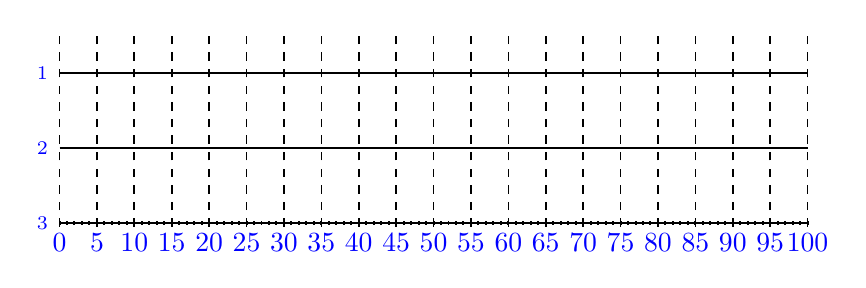
\begin{tikzpicture}[
		scale=0.095,
		line width=0.25mm,
		every node/.style={scale=1, text=blue},
		major tick/.style={semithick, dashed},
		x tick label/.style={anchor=north, minimum width=5mm},
		task1/.style={blue},
		task2/.style={red},
		task3/.style={green},
		desc/.style={anchor=east}
		]		

	% Task 1
	\draw (0, 20) -- (100, 20);
	\node[desc] at (0, 20) {$\uptau_1$};		
	
	% Task 2
	\draw (0, 10) -- (100, 10);
	\node[desc] at (0, 10) {$\uptau_2$};	
	
	% Task 3
	\draw (0, 0) -- (100, 0);
	\node[desc] at (0, 0) {$\uptau_3$};	
	
	% Small ticks
	\foreach \x in {0, 1,...,100}{
		\draw (\x, -0.25) -- (\x, 0.25);
	}
	
	% Major ticks with label
	\foreach \x/\label in {0, 5,...,100}{
		\node[x tick label] at (\x, 0) {$\label$}; 		
		\draw[major tick] (\x, -0.5) -- (\x, 26);
	}
	
%	\draw[task1] (0, 20) -- (0, 25) -- (5, 25) -- (5, 20);
%	\draw[task2] (5, 10) -- (5, 15) -- (10, 15) -- (10, 10);
%	\draw[task3] (10, 0) -- (10, 5) -- (15, 5); % 5 of 7
%	\draw[task1] (15, 20) -- (15, 25) -- (20, 25) -- (20, 20);
%	\draw[task2] (20, 10) -- (20, 15) -- (25, 15) -- (25, 10);
%	\draw[task3] (25, 5) -- (27, 5) -- (27, 0); % 7 of 7
%	\draw[task1] (30, 20) -- (30, 25) -- (35, 25) -- (35, 20);
%	\draw[task2] (35, 10) -- (35, 15) -- (40, 15) -- (40, 10);
%	\draw[task3] (40, 0) -- (40, 5) -- (45, 5); % 5 of 7
%	\draw[task1] (45, 20) -- (45, 25) -- (50, 25) -- (50, 20);
%	\draw[task2] (50, 10) -- (50, 15) -- (55, 15) -- (55, 10);
%	\draw[task3] (55, 5) -- (57, 5) -- (57, 0); % 7 of 7
%	\draw[task1] (60, 20) -- (60, 25) -- (65, 25) -- (65, 20);
%	\draw[task2] (65, 10) -- (65, 15) -- (70, 15) -- (70, 10);
%	\draw[task3] (70, 0) -- (70, 5) -- (75, 5); % 5 of 7
%	\draw[task1] (75, 20) -- (75, 25) -- (80, 25) -- (80, 20);
%	\draw[task2] (80, 10) -- (80, 15) -- (85, 15) -- (85, 10);
%	\draw[task3] (85, 5) -- (87, 5) -- (87, 0); % 7 of 7
%	\draw[task1] (90, 20) -- (90, 25) -- (95, 25) -- (95, 20);
%	\draw[task2] (95, 10) -- (95, 15) -- (100, 15) -- (100, 10);

		
	\end{tikzpicture}
%	\caption{Ablaufübersicht}
\end{figure} 